\chapter{Bluetooth Proximity}
\label{chap:bt_proximity}

\section{Background}
Interactions are not limited to any particular area and can take place at a wide variety of locations, ranging from sitting and chatting in a Starbucks coffee shop to walking and chatting across a college campus. As will be explored later in the paper, for most face-to-face interactions, the approximate distance between individuals in casual conversation is within 0.5 to 2.5 meters. One of the solutions would seem to be location-based calculation which relies on location technologies such as WiFi triangulation~\cite{wifi}, cell phone triangulation~\cite{cell}, GPS, or a combination of all three. However, none of these solutions are ideal or sufficient. Although WiFi triangulation can present a reasonable degree of accuracy, its accuracy in all but the most dense WiFi deployments is insufficient, ranging on the order of 3 to 30 meters~\cite{wifi}. Similarly, cell phone triangulation suffers from an even worse accuracy~\cite{cell}. Moreover, while WiFi is reasonably pervasive, WiFi tends to generally be sparser in green spaces, i.e. outdoor spaces. Notably, GPS suffers from both an accuracy shortcoming (5-50m) as well as a lack of viability indoors~\cite{survey1}. 

However, it is important to note that face-to-face interaction does not demand an absolute position as offered by the previously mentioned schemes but rather requires a determination of \textit{proximity}. With that important shift of the problem definition, Bluetooth emerges as a straightforward and plausible alternative, offering both accuracy (1-1.2m)~\cite{BTposition} and ubiquity (most modern smartphones come with Bluetooth)~\cite{Nathan2}. Although some prior work has attempted to use the detection of Bluetooth to indicate nearness~\cite{Nathan3}, it is not enough for the face-to-face proximity estimation. The question addressed by this section is to what extent Bluetooth can be an accurate estimator of such proximity.  

\section{Related Work}\label{sec:related work}
Over the years, there has been a number of technologies proposed for proximity detection. Approaches such as those used by Meme Tags~\cite{borovoy1998meme} provide good accuracy but require line of sight. Ultrasound approaches such as Activebadge ~\cite{want1992active} also provide good accuracy but they require infrastructure support. ZigBee technology is widely used in wireless sensor network to provide radio proximity estimation~\cite{baouche2009radio} in the environment where GPS is inoperative. Proximity can also be reported by sounds, and past work has shown audio to be effective for delivering peripheral cues~\cite{mynatt1997audio}. However, it is untenable to expect the use of smartphones to reduce the unobtrusiveness of cues or increase comprehension. For the purposes of this paper, we are interested in techniques that are based on commonly available technologies in smartphones, i.e. GPS, Cell, WiFi and Bluetooth. Particularly, we are interested in techniques that can be applied at the smartphone itself without significant changes to the infrastructure. 

Proximity detection is one of the advanced Location based Service (LBS) functions~\cite{treu2005efficient,kupper2006efficient,vsikvsnys2010private} to automatically detect when a pair of mobile targets approach each other closer than a predefined proximity distance (as in Location Alerts of Google Latitude). For realizing this function the targets are equipped with a cellular mobile device with an integrated GPS receiver, which passes position fixes obtained by GPS to a central location server. Most proposals for such services give low accuracy guarantees and incur high communication costs. Recently, 3-D optical wireless based location approach~\cite{bilgi20103} is proposed which based on both GPS and triangulation technologies. It is another feasible way of utilizing GPS to get relative distance among objects. 

Some proximity estimation methods are based on Cell or WiFi signal. Using Place Lab~\cite{lamarca2005place}, cell phones listen for the MAC address of fixed radio beacons, such as cell tower and wireless access points, and reference the beacons� positions in a cached database. It provides adequate accuracy for detecting something like buddy proximity (e.g., median accuracy of 20-30 meters), but it requires a �wardriving� of the area to obtain pre-mapped cell towers and fixed wireless APs in the area. This can be quite costly, especially keeping the information up to date, as tower positions, etc. are updated on an annual basis. Without calculating absolute location, NearMe~\cite{krumm2004nearme} explores the algorithm for detecting proximity using Wi-Fi signatures (WiFi APs and signal strengths), allowing it to work with no a priori setup. Similarly, ~\cite{li2008peopletones} uses GSM readings to explore the proximity of mobile targets. 

There are some proximity detection works using Bluetooth signal. From a specific work perspective, the works of Nathan et al. ~\cite{Nathan3,Nathan1} are highly relevant to the paper. In those studies, the authors use the ability to detect Bluetooth signals as indicators for people nearby within the Bluetooth range (around 10m). However, such indication does not meet the requirement of face-to-face proximity detection. In class, a student may discuss with others sitting beside him/her, but face-to-face talk is difficult with the students on the other side of the classroom even they are still in the Bluetooth range. Different from the above proximity detection method, our work is a fine grain Bluetooth-based proximity detection method which can provide adequate accuracy for face-to-face proximity estimation without environment limitations. Table~\ref{table:comparison} summarizes the differences of popular techniques, their prominent features and the performance~\cite{survey2,MobileLocation}. 

\begin{table}[ht] 
\caption{DIFFERENT PROXIMITY ESTIMATION TECHNIQUES COMPARISON} 
\centering  
\begin{tabular}{lccc}
\hline
  &Bluetooth & WiFi & GPS \\ [0.5ex] 
\hline\hline HW costs & Medium & High & High\\ 
\hline Coverage & High & High(Indoor) & High (Outdoor)\\
\hline Power Usage & Medium & High & High\\
\hline Accuracy & 1-4m & 2-30m & 5-50m \\
\hline Security & High & High & Not applicable \\	
\hline
\end{tabular}
\label{table:comparison} 
\end{table}

Based on the monitoring system described in Chapter~\ref{chap:dataset}, there are more than one million Bluetooth records collected per week. Figure~\ref{fig:multiphones} shows the distribution of the Bluetooth RSSI values collected from 196 phones in one week (more details will be discussed in Section~\ref{sec:exp} and Section~\ref{sec:case}). The data collected includes both indoor and outdoor environments. As it shows,  the most prevalent value is around -76dBm which indicates much more than 5m indoor and nearly 5m outdoor as will be shown later. Therefore, an unfiltered detection method such as ~\cite{Nathan3,Nathan1} is not enough to estimate the face-to-face proximity and we use a more accurate method in Section~\ref{sec:exp} to solve this problem. Moreover, we introduce various smoothing effects and take advantage of empirical observations to function across a wide variety of typical environments. 

\begin{figure}[h!tbp]
\centering
{\includegraphics[width=4in]{graphs/Figure2.eps}}
\caption{Bluetooth RSSI Values Distribution in One Week} 
\label{fig:multiphones}
\end{figure}

\section{Proximity Estimation Model}\label{sec:exp}
In this section, we explore the relationship between Bluetooth RSSI and distance in real world scenarios. The first method is using RSSI value threshold to determine whether two phones are in proximity or not. The second method introduces the light sensor data to determine whether the phone is indoors or outdoors, inside the backpack or in hand. By differentiating environments and smoothing data, a face-to-face proximity estimation model is outlined to improve the estimation accuracy in general scenarios. At the end of this section the proximity accuracy of Bluetooth, WiFi and GPS are analyzed and compared. 

\subsection{Bluetooth RSSI vs. Distance}
Antti et al. presented the design and implementation of a Bluetooth Local Positioning Application (BLPA)~\cite{BLPA} in which the Bluetooth received signal power level is converted to distance estimate according to a simple propagation model as follows: 
\begin{flalign}
\begin{split}
RSSI  &= P_{TX} + G_{TX} + G_{RX} + 20\log{(\frac{c}{4\pi f})} - 10n\log{(d)}\\
	&= P_{TX} + G -40.2 - 10n\log{(d)}
\end{split}&
\end{flalign}
where \( P_{TX}\) is the transmit power; \(G_{TX}\) and \(G_{RX}\) are the antenna gains; G is the total antenna gain: \(G = G_{TX} + G_{RX}\); \(c\) is the speed of light (\(3.0 * 10^{8}m/s\)); \(f\) is the central frequency (2.44 GHz); \(n\) is the attenuation factor (2 in free space); and \(d\) is the distance between transmitter and receiver (in m). \(d\) is therefore:
\begin{flalign}
\begin{split}
\label{equation: d}
d = 10^{[(P_{TX} - 40.2 - RSSI + G) / 10n]}
\end{split}&
\end{flalign}
However, such a model can only be utilized as a theoretical reference. Due to reflection, obstacles, noise and antenna orientation, the relationship between RSSI and distance becomes more complicated. Our challenge was to assess how much impact these environmental factors have on Bluetooth RSSI values. Therefore, we carried out several experiments to understand how the Bluetooth indicators fade with distance under these environmental influences. 

Indoor experiments were conducted in a noisy hallway (around seven other Bluetooth devices detected) in the campus engineering building. Outdoor experiments were conducted in the open area outside the building. In the measurement there were no obstacles between the two phones and the antennas of the phones were aligned towards each other. In such a way, we tried to build up a relatively simple and ``ideal'' environment where the possible impact factors are reflection and noise only. We repeated the measurements over the period of an hour with the distance being increased by 0.5 meters between each round. Figure~\ref{fig:RSSI} shows the initial fluctuations of indoor RSSI results with different distances. Although the data varies significantly even within the same distance, there is a noticeable gap exists between different distances. Such results further shed light on the viability of using Bluetooth RSSI to indicate the face-to-face proximity.
\begin{figure}[h!tbp]
\centering
{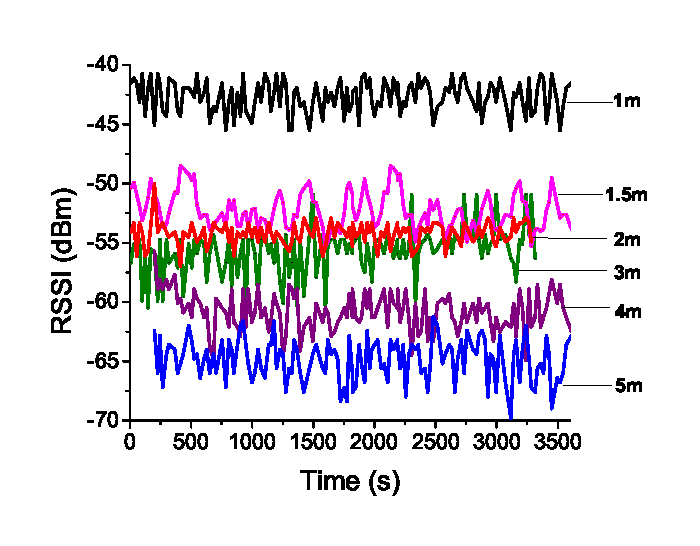
\includegraphics[width=4in]{graphs/Figure4.eps}}
\caption{Initial Indoor RSSI Values with Different Distances} 
\label{fig:RSSI}
\end{figure}

In Figure~\ref{fig:theory}, we present indoor, outdoor, and theoretical results for Bluetooth across a variety of distances (0-5 meters). The theoretical values were predicted by the propagation model with \(P_{TX}=2.9\ dBm\) and \(G=4.82\ dBi\). These specific values are the average empirical results of our experiment phone. We calculated the average RSSI from nearly 120 raw values for each distance. The indoor results were relatively close to the theoretical values. However, the results outside the building were much farther away from the theoretical reference and imply that these two kinds of environmental settings should be identified in the following measurements.
\begin{figure}[h!tbp]
\centering
{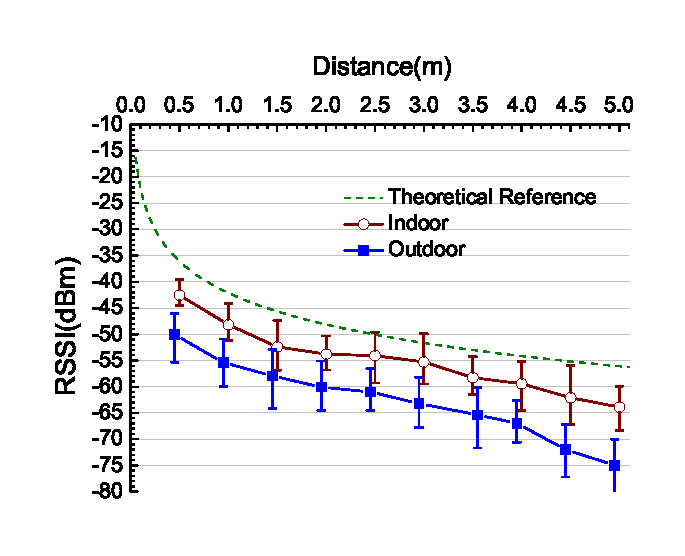
\includegraphics[width=3.5in]{graphs/Figure5.eps}}
\caption{Bluetooth RSSI vs. Distance - Theoretical, Indoor \& Outdoor} 
\label{fig:theory}
\end{figure}

Furthermore, we performed similar experiments on two phones focusing on the indoor case but with different antenna orientation (e.g. in the same direction) and obstacles (e.g. put in a backpack or partitioned by cubicle) in order to discover the influence of these possible factors. Figure~\ref{fig:inside} illustrates the results with these impacts. The observations include the following: first, the change in orientation turns out to have little impact on the final results. As many smart phones cannot predict phone orientation, antenna design is typically optimized to account for this fact. Second, although we placed two phones on each side of a cubicle board, such an arrangement did not affect RSSI significantly. Third, the most important environmental issue came from the backpack. It may be because the signal of Bluetooth is disturbed or shielded in such a closed environment. As many individuals would be likely to carry their phone in a purse or backpack (particularly on a college campus), the backpack setting bears further investigation. We also recorded the data to check whether the RSSI values on phones are symmetric. Figure~\ref{fig:inside_reverse} shows the RSSI values on one phone are almost the same as the results on the other phone. 
\begin{figure}[h!tbp]
\centering
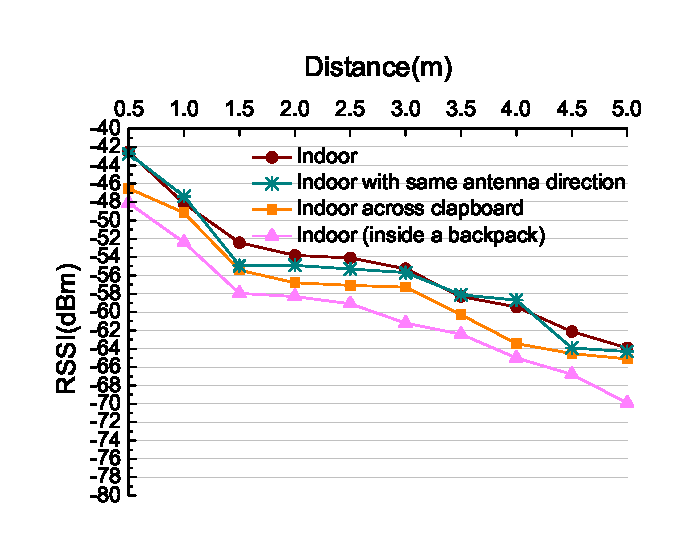
\includegraphics[width=3.5in]{graphs/Figure6.eps}
\caption{Bluetooth RSSI vs. Distance Indoor Case} 
\label{fig:inside}
\end{figure}

\begin{figure}[h!tbp]
\centering
\includegraphics[width=3.5in]{graphs/Figure7.eps}
\caption{Symmetric RSSI Values} 
\label{fig:inside_reverse}
\end{figure}

Using the same method, we measured the RSSI values outdoors with the consideration of the influence of a backpack. Figure~\ref{fig:outside} shows the results from those experiments. Similarly, the RSSI values become lower when the phones are in the backpack so it is a non-ignorable element in the following estimations, further reinforcing that detection of such an arrangement may be critical for proper distance estimation resolution.

\begin{figure}[h!tbp]
\centering
\includegraphics[width=3.5in]{graphs/Figure8.eps}
\caption{Bluetooth RSSI vs. Distance Outdoor Case} 
\label{fig:outside}
\end{figure}

Based on these indoor and outdoor results, there are two main environmental factors that may effect the RSSI values: inside/outside building and inside/outside a backpack. Besides those factors, it is also necessary to take multiple-phones scenario into consideration since phones with Bluetooth around may have interference on Bluetooth RSSI values. 

\subsection{Proximity Estimation Model}
As mentioned in the beginning, we aim to provide an accurate proximity estimation for face-to-face communication. This raises a question: what is the face-to-face communication distance? In this subsection, we first define the face-to-face distance and then use the indoor results as a threshold to do the estimation in real world scenarios. Since the error rate of using a simple threshold is relatively high, we explore the possible reasons and propose a proximity estimation model with the introduction of light sensor values. 

\emph{Distance of face-to-face communication:}
When we have dinner with our friends sitting at the same table, the conversation among us is called face-to-face communication; or when we talk with someone side by side, the distance between us is also called face-to-face communication. In other words, face-to-face communication happens when people are close enough to have conversations in a convenient manner. People typically have such communication when they are sitting or walking together. Thus, we calculate the distance for this kind of communication by measuring distances across the campus (such as diagonal of desk in dinning hall, distance between desks in classrooms and etc.) and the average value is equal to 1.52m. The detailed samples are listed in Table~\ref{table:distance}. 

\begin{table}[ht] 
\caption{DISTANCE OF FACE-TO-FACE COMMUNICATION AROUND CAMPUS} 
\centering  
\begin{tabular}{lccc}
\hline
\multicolumn{1}{c}{Place} & Distance(cm) \\ [0.6ex] 
\hline\hline Diagonal of small square desk in La Fortune & 116\\ 
\hline Diagonal of large square desk in La Fortune & 160\\
\hline Diameter of round desk in La Fortune & 120\\
\hline Diagonal of desk in dinning hall & 250\\
\hline Distance between desks in Cushing office & 125\\
\hline Distance between desks in classroom & 155\\
\hline Diagonal of desk in discussion cubic & 220\\
\hline Distance between people walking side by side & 70\\	
\hline
\end{tabular}
\label{table:distance} 
\end{table}

To conduct an evaluation of the accuracy of our Bluetooth method, we constructed a scenario that draws upon several likely occurrences in normal campus interactions. The scenario blends each of the earlier test cases and provides data to assess the accuracy in a real-world setting. 
The measurement was conducted as follows: two people with two phones walked side by side from Cushing Hall to Grace Hall and then returned back (Figure~\ref{fig:map}).

\begin{figure}[h!tbp]
\centering
{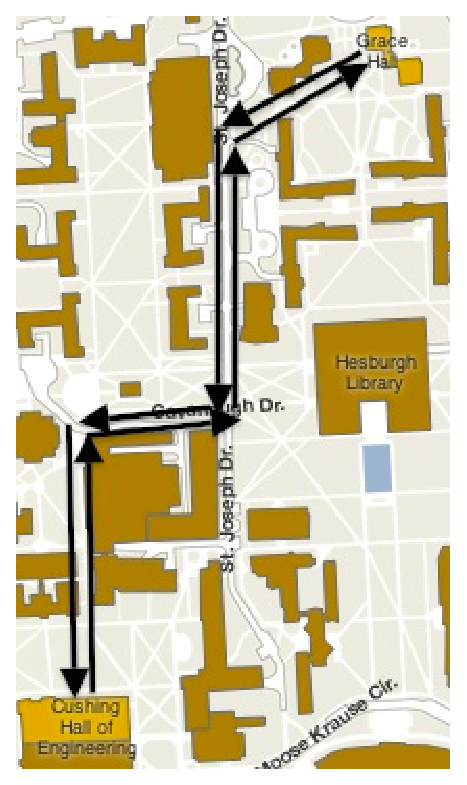
\includegraphics[width = 2.2in]{graphs/Figure9.eps}}
\caption{Walk Path for Real-world Scenario} 
\label{fig:map}
\end{figure} 

The whole process took 40 minutes and individuals were always within the distance for face-to-face communication. The Bluetooth update time interval was changed to 10 seconds temporarily in order to provide enough samples. During the first ten minutes (phone in hand) and last ten minutes (phone inside a backpack) individuals were inside Cushing Hall. When individuals were outside (the duration was 20 minutes), in the first ten minutes individuals held the phones in their hands and then put the phones in their backpack for the later ten minutes. 

\emph{Single Threshold:} 
After data collection, the corresponding RSSI value (-52dBm) of direct communication distance (152cm) based on the indoor measurements (Figure~\ref{fig:inside}) was used as a threshold to estimate whether the individuals were in proximity. Accordingly, values less then \mbox{-52dBm} were considered as not in face-to-face proximity and labeled as a wrong estimation.

\begin{table}[ht] 
\caption{ERROR RATE AGAINST REAL-WORLD DATA} 
\centering  
\begin{tabular}{lccc}
\hline\hline 
Total samples & 246 \\ [0.6ex] 
\hline Total error rate & 72.8\%\\ 
\hline Indoor error rate (0 - 10 mins) & 14.3\%\\
\hline Outdoor error rate (10 - 20 mins) & 91.3\%\\
\hline Outdoor (inside a backpack) error rate (20 - 30 mins) & 100.0\%\\
\hline Indoor (inside a backpack) error rate (30 - 40 mins)  & 85.0\%\\	
\hline
\end{tabular}
\label{table:naive} 

\end{table}
\begin{table}[ht] 
\caption{IMPROVED ERROR RATE WITH MODIFIED THRESHOLD} 
\centering  
\begin{tabular}{lccc}
\hline\hline 
Total samples & 246 \\ [0.6ex] 
\hline Total error rate & 48.4\%\\ 
\hline Indoor error rate (0 - 10 mins) & 4.9\%\\
\hline Outdoor error rate (10 - 20 mins) & 53.2\%\\
\hline Outdoor (inside a backpack) error rate (20 - 30 mins) & 85.5\%\\
\hline Indoor (inside a backpack) error rate (30 - 40 mins)  & 49.2\%\\	
\hline
\end{tabular}
\label{table:naive2} 
\end{table}

Table~\ref{table:naive} shows the results and error rate of this na\"{\i}ve method. It was found that both of the outdoor and backpack parts have extremely high error rates. After switching the threshold value to -58dBm which is the outdoor RSSI values with 152cm distance,  the error rate was improved but still high as shown in Table~\ref{table:naive2}.

In our opinion, the reasons for high error rates include: 
\newline i) One fixed threshold is not enough as the indicator of correct or wrong estimation; 
\newline ii) Only indoor or outdoor relationship was used to analyze the data without differentiation; 
\newline iii) The influence of backpack and other possible environmental interference were not taken into consideration; 
\newline iv) Each RSSI value was not smoothed to allow for environmental fluctuations.

\emph{Multiple Thresholds:} 
According to the reasons for high error rate analyzed above, we introduce the proximity estimation model which is a multiple threshold-based method with the consideration of data smoothing and different environmental effects.

i) Data Smoothing

Since there is time delay during the data collection, we do smoothing on the data collection to avoid environmental fluctuation effects and there are several ways to achieve it. One way is using simple window function and each value \(RSSI_{i}\) at time \(i\) is modified using the following function:
\begin{flalign}
\begin{split}
RSSI_{i}=a* RSSI_{i-1} + b* RSSI_{i} + c* RSSI_{i+1}
\end{split}&
\end{flalign}
For the values of the parameters (a, b and c), several combinations such as (0.4, 0.6, 0), (0.3, 0.4, 0.3) and (0.2, 0.6, 0.2) are used in the following comparisons. 
Another smoothing method is to utilize EWMA (exponentially weighted moving average) to analyze the dataset. Let \(E_{i}\) be the EWMA value at time \(i\) and \(s\) be the smoothing factor. The EWMA calculation is as follows:
\begin{flalign}
\begin{split}
E_{i}=s* RSSI_{i} + (1-s)E_{i-1}
\end{split}&
\end{flalign}
Based on real-world data as shown in Table~\ref{table:naive2}, we combine the data smoothing method with signal threshold filter to analyze the effects of data smoothing and select the best smoothing function. In Table~\ref{table:smoothing}, we compare three different combinations for window function and two types of smoothing factors. While the combination (0.3, 0.4, 0.3) exhibits good improvement of error rate in different scenarios compared with results in Table~\ref{table:naive2}, the EWMA methods with smoothing factor 0.5 is the best among the five options and we use it in the proximity estimation model.

\begin{table}[ht] 
\caption{IMPROVED ERROR RATE WITH DATA SMOOTHING} 
\centering
\begin{tabular}{|c|c|c|c|c|c|}
\hline 
& \multicolumn{3}{c|}{Simple Window Function} & \multicolumn{2}{c|}{EWMA}\\
\hline
& (0.4, 0.6, 0) & (0.3, 0.4, 0.3) & (0.2, 0.6, 0.2) & s = 0.5 & s = 0.8\\
\hline Total& 49.6\% & 28.3\% & 37.1\% & 26.8\% & 38.2\%\\ 
\hline Indoor & 5.4\% & 3.4\% & 5.7\% & 2.1\% & 4.9\%\\
\hline Outdoor & 50.8\% & 39.4\% & 42.3\% & 23.8\% & 34.7\%\\
\hline Outdoor backpack & 82.9\% & 59.3\% & 76.8\% & 61.2\% & 79.1\%\\
\hline Indoor backpack & 50.7\% & 30.2\% & 45.7\% & 27.5\% & 48.3\%\\	
\hline
\end{tabular}
\label{table:smoothing} 
\end{table}

ii) Light Sensor Data

As shown in Figure~\ref{fig:inside} and Figure~\ref{fig:outside}, the Bluetooth RSSI values are much smaller than the indoor ones when the phone is in the backpack or outdoors. One of our observations is that it is possible to treat the light sensor data as an indicator of the environment. Figure~\ref{fig:light} reveals the light sensor data distribution in different settings: during the daytime when the phone is inside the building the light sensor returns values between 225 to 1280; while this value comes up to larger than 1280 when phone is under daylight. When the phone is in the backpack, the light values are typically around 10.  Therefore, when the light sensor value is in a range that indicates the phone is in a specific corresponding environment. 

In Figure~\ref{fig:walkdata}, we reviewed the distribution of the Bluetooth RSSI values collected in the walk experiment and the corresponding light sensor data got at the same time. As shown, there is RSSI data fluctuation even in the same setting due to the interference and noise. However, most Bluetooth RSSI values are larger than -55dBm when light sensor data is from 225 to 1280 (indicates indoor setting) while the RSSI values are smaller than -55dBm when light sensor data is in other zones (either in the backpack or outdoors). 

\begin{figure}[h!tbp]
\centering
{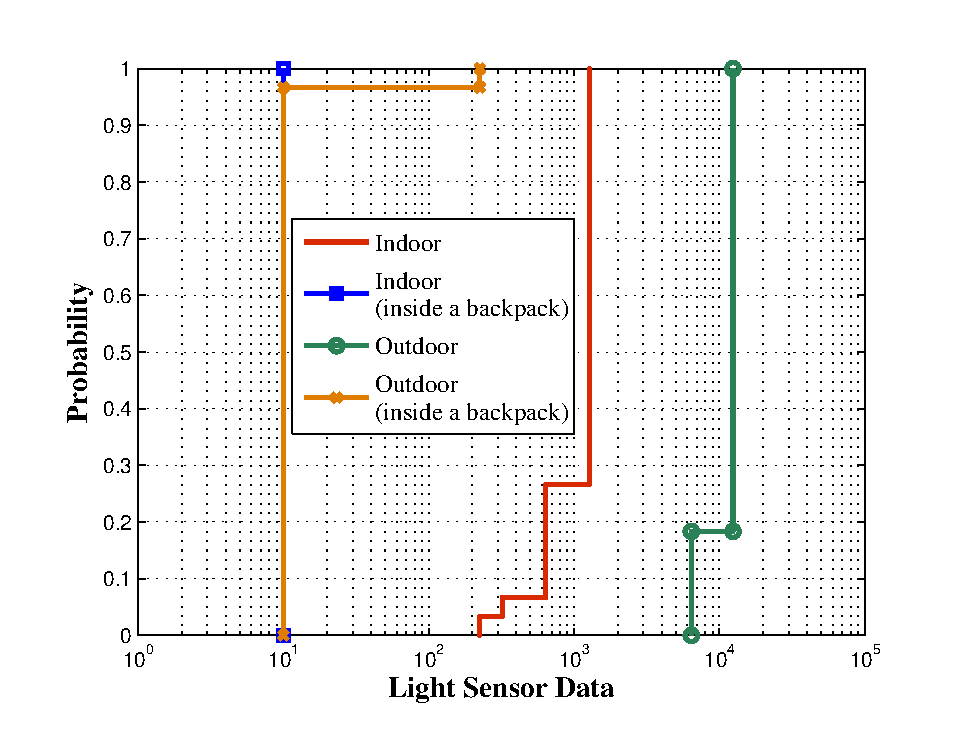
\includegraphics[width=3.5in]{graphs/Figure10.eps}}
\caption{Cdf of Light Sensor Data in Different Environments} 
\label{fig:light}
\end{figure} 

\begin{figure}[h!tbp]
\centering
{\includegraphics[width=3.5in]{graphs/Figure11.eps}}
\caption{Data in Real-world Scenario} 
\label{fig:walkdata}
\end{figure} 

Thus, light sensor data is introduced to differentiate the circumstances to improve the accuracy of distance estimation based on the rules in Table~\ref{table:light}. Variations due to time of day (day vs. evening) may be accounted for using the smartphone time. Inevitably, accuracy will decrease during evening hours but we felt this is an adequate tradeoff for improved environmental detection. Unfortunately, the Nexus S 4G phone does not contain a pressure sensor which could be used to further improve results.  

\begin{table}[ht] 
\centering
\caption{ENVIRONMENT ESTIMATION WITH LIGHT SENSOR DATA}
\begin{tabular}{cc}
\hline\hline 
Light Sensor Data & Environment Estimation\\ [0.3ex] 
\hline (0, 100] & Inside backpack\\
\hline (100, 1280] & Indoor and out of backpack\\
\hline $>$1280 & Outdoor and out of backpack\\
\hline
\end{tabular}
\label{table:light} 
\end{table}

iii) Proximity Estimation Model

Based on the analysis of noise and interference, we use a multiple threshold model instead of a single threshold to do the proximity estimation. In Figure~\ref{fig:theory}, the corresponding indoor RSSI values of 2.5m (the maximum distance for face-to-face communication) is around -55dBm. It is obvious that when the received RSSI value is larger than -55dBm the two phones are in face-to-face proximity. Similarly, when the outdoor RSSI values is larger than -60dBm the two phones holder are close enough to have direct interaction. We call such data zone the \textit{``Positive Zone"} denoting where two individuals are certainly within face-to-face interaction distance.

For the indoor data smaller than -55dBm, the model is constructed based on the following observation: in Figure~\ref{fig:inside} the smallest value for 5m distance in the test was -65dBm and it had a relatively low probability of occurence (values larger than -65dBm is less than 20\%) in Figure~\ref{fig:multiphones}. Taking noise and interference into consideration, the value between -65dBm and -55dBm may also indicate a face-to-face proximity with high probability. Figure~\ref{fig:multiphones} includes both indoor and outdoor data and the most frequent data is -76dBm and the lowest values detected is -90dBm. When the indoor data is in (-76dBm, -65dBm), it is still possible to make a face-to-face communication but the probability is relatively low. The indoor data smaller than -76dBm implies that it is too far to have a direct communication and it is called the \textit{``Negative Zone"}. Similarly, we set up several bounds for outdoor data: the smallest value for 5m is -75dBm. Therefore the zone(-75dBm, -60dBm) has a relatively high probability while the zone(-90dBm, -75dBm) is the low probability zone. When the outdoor data is smaller than -90dbm, we strongly believe it is impossible to indicate a face-to-face proximity or even be detected. 

Furthermore, we revisit the data regarding the inside backpack environment. Based on light sensor data, it is difficult to distinguish indoor or outdoor when the phone is inside the backpack. We noticed that when distance are 2.5m and 5m, the corresponding indoor Bluetooth RSSI values inside a backpack are -59dBm and -70dBm and the corresponding outdoor values are -64dBm and -79dBm. We defined the zone which is larger than -59dBm as \textit{``Positive Zone"} for backpack data. Similarly, the zone which is smaller than -79dBm as \textit{``Negative Zone"}. For the data between the two above bounds, we also define \textit{``High Probability (HP) Zone"} (-70dBm, -59dBm) and \textit{``Low Probability (LP) Zone"} (-79dBm, -70dBm). Therefore, for each type of environment, we have four zones as summarized in Table~\ref{table:distribution}. Table~\ref{table:multithresholds} lists the corresponding multiple thresholds. Figure~\ref{fig:distribution} illustrates the multiple thresholds of different zones in a more direct way. 

For high and low probability zones, we name the minimum values in low probability zone as \textit{B$_{min}$}, the maximum value in high probability zone as \textit{B$_{max}$} and the range as \textit{B$_{range}$}. Therefore B$_{range}$ = B$_{max}$ - B$_{min}$. To sum up, a proximity estimation model with multiple thresholds is proposed to improve the accuracy. For Bluetooth RSSI value \textit{x$_i$} and the corresponding light sensor value \textit{y$_i$} at time \textit{i}, we calculate the probability of face-to-face proximity \textit{p$_i$} as described in algorithm~\ref{algo:procedure}.

\begin{table}[ht] 
\centering
\caption{DEFINITION OF ZONES IN DIFFERENT ENVIRONMENTS} 
\begin{tabular}{lccc}
\hline\hline 
Zones &  Indoor & Outdoor & Inside Backpack \\ [0.3ex] 
\hline Positive & $>$=B$_{I\_FTF}$ & $>$=B$_{O\_FTF}$ & $>$=B$_{I\_P\_FTF}$\\
\hline HP & [B$_{I\_5m}$, B$_{I\_FTF}$) & [B$_{O\_5m}$, B$_{O\_FTF}$) & [B$_{I\_P\_5m}$, B$_{I\_P\_FTF}$)\\
\hline LP & [B$_{frequent}$, B$_{I\_5m}$) & [B$_{min}$, B$_{O\_5m}$) & [B$_{O\_P\_5m}$,B$_{I\_P\_5m}$)\\
\hline Negative & $<$B$_{frequent}$ & $<$B$_{min}$ & $<$B$_{O\_P\_5m}$\\
\hline
\end{tabular}
\label{table:distribution} 
\end{table}

\begin{table}[ht] 
\centering
\caption{BOUNDARY SUMMARY}
\begin{tabular}{llc}
\hline\hline 
Boundary &  \multicolumn{1}{c}{Detail} & Values(dBm) \\ [0.3ex] 
\hline B$_{I\_FTF}$& Indoor fact-to-face (2.5m) & -55\\
\hline B$_{O\_FTF}$& Outdoor fact-to-face (2.5m) & -60\\
\hline B$_{I\_P\_FTF}$& \parbox[t]{3cm}{Indoor inside backpack fact-to-face (2.5m)} & -59\\
\hline B$_{O\_P\_FTF}$& \parbox[t]{3cm}{Outdoor inside backpack fact-to-face (2.5m)}& -64\\
\hline B$_{I\_5m}$& Indoor 5m & -65\\
\hline B$_{O\_5m}$& Outdoor 5m & -75\\
\hline B$_{I\_P\_5m}$& Indoor inside backpack 5m & -70\\
\hline B$_{O\_P\_5m}$& Outdoor inside backpack 5m & -79\\
\hline B$_{frequent}$& Most frequent value in the results& -76\\
\hline B$_{min}$& Minimum in the results & -90\\
\hline
\end{tabular}
\label{table:multithresholds} 
\end{table}

\begin{figure}[h!tbp]
\centering
{\includegraphics[width=6in]{graphs/Figure12.eps}}
\caption{Multiple Thresholds in Different Zones} 
\label{fig:distribution}
\end{figure} 

\begin{algorithm}
\caption{Estimate probability $p_i$ of face-to-face proximity with Bluetooth RSSI value $x_i$ and light sensor value $y_i$}
\begin{algorithmic} 
\STATE $x_i \leftarrow a*x_{i-1} + b*x_i + c*x_{i+1}$
\STATE determine the scenario depending on $y_i$
\IF{$x_i\ is\ in\ positive\ zone$}
\STATE $p_i \leftarrow 1$
\ELSIF{$x_i\ is\ in\ probability\ zone\ [B_{min}, B_{max})$}
\STATE $p_i \leftarrow (x_i-B_{min})/B_{range}$
\ELSE
\STATE $p_i \leftarrow 0$
\ENDIF
\end{algorithmic} 
\label{algo:procedure} 
\end{algorithm}

We define \textit{Required Accuracy} (RA) as the lowest requirement for the probability to indicate two phones are in face-to-face proximity. With the improved estimation model, we analyze the data in the real-world scenario again and the error rate is improved greatly as shown in Table~\ref{table:improved}. Once \textit{p$_i$} is higher than 45\% ( RA = 45\%), the two phones are considered to be in the face-to-face proximity. The bigger the RA value is, the more accurate face-to-face proximity we can obtain. We choose 45\% as RA based on the following calculation: in each type of environment, the probability of the lowest possible value \textit{l} in high probability zone equals to (l-\textit{B$_{min}$}) divided by \textit{B$_{range}$}. The smallest one in three types of environments equals to 45\%.

\begin{table}[ht] 
\caption{ERROR RATE AGAINST REAL-WORLD DATA WITH PROXIMITY ESTIMATION MODEL} 
\centering  
\begin{tabular}{lccc}
\hline\hline 
Total samples & 246 \\ [0.5ex] 
\hline Total error rate & 4.3\%\\ 
\hline Inside error rate (0 - 10 mins) & 0.0\%\\
\hline Outside error rate (10 - 20 mins) & 4.5\%\\
\hline Outside (inside a backpack) error rate (20 - 30 mins) & 8.3\%\\
\hline Inside (inside a backpack) error rate (30 - 40 mins)  & 6.2\%\\
\hline
\end{tabular}
\label{table:improved} 
\end{table}

\subsection{Comparisons}

WiFi triangulation/trilateration is a widely used method to do location indoors while GPS is perhaps the most popular way to do location outdoors. As summarized in Section~\ref{sec:related work}, both of them have their own advantages and disadvantages. Here we use WiFi and GPS to do the face-to-face proximity estimation in order to compare the accuracy of them with the Bluetooth method we proposed. Together with the power consumption comparison in Section~\ref{sec:system}, the method of Bluetooth is proved to be an effective and efficient way in both aspects of accuracy and power usage. 

We collected both network-provider location and GPS location data on the phone for the comparison. With the API provided by class \textit{LocationManager} in Android SDK, we can get both kinds of location data by choosing different location providers with the frequency of three minutes. The GPS provider determines location using satellites while the network provider determines location based on availability of cell tower and WiFi access points(APs). In the network provider method, the triangulation is used to get the location of the phone with the knowledge of cell towers' or APs' locations. When each phone's location is known, the relative distance as well as the accuracy is easy to calculate. 
\newline\indent We conducted the experiment on a game day in the campus. Two students (A and B) went to Notre Dame Stadium to watch the game together. In Figure~\ref{fig:wifi_gps} the reported location data are marked. From 3pm to 7pm, the location data recorded by network provider are (41.699517, -86.232877) and (41.699203, -86.235269). During the same time period, the GPS provider collected the location as (41.699504, -86.234624) and (41.699004, -86.235723). The corresponding distance between the reported data were 11.25 meters (443 inches) and 7.92 meters (312 inches) respectively. Based on the results reported by the phones, the accuracy of WiFi-based localization turns out to be around 10-15 meters and the one using GPS is around 10 meters. 

\begin{figure}[h!tbp]
\centering
{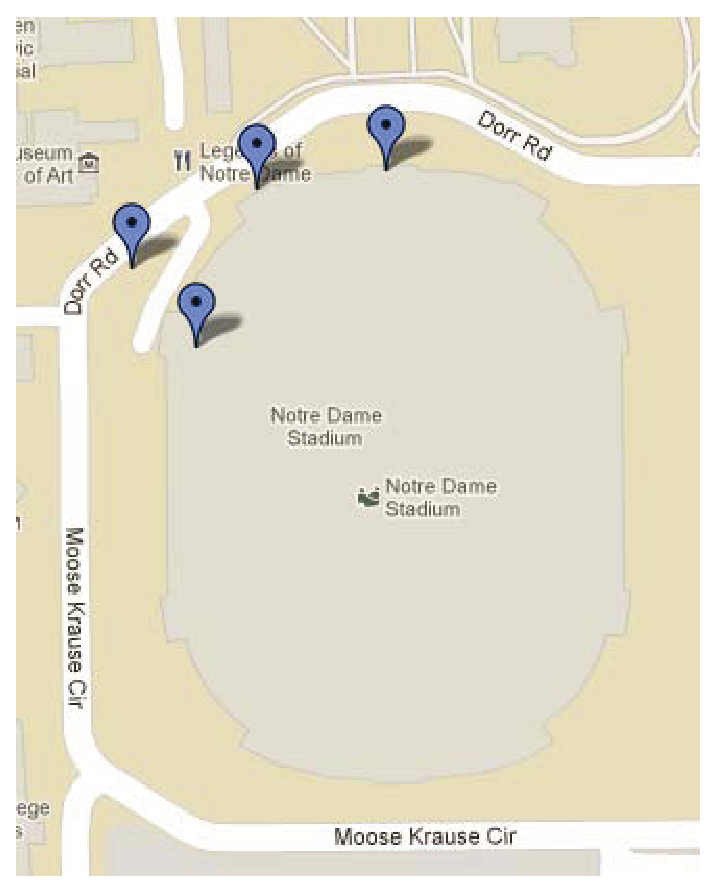
\includegraphics[width=2.5in]{graphs/Figure13.eps}}
\caption{Location Data Provided by WiFi and GPS} 
\label{fig:wifi_gps}
\end{figure} 

Compared to the above WiFi triangulation and GPS methods, the Bluetooth-based method was more suitable for the face-to-face proximity estimation. As we mentioned before, there is no need to get the absolute location data to calculate the distance. Instead, we only need relative distance to do the estimation. From 3pm to 7pm on that day, we collected the Bluetooth RSSI on both phones and used the estimation model to do the analysis. When RA is 45\%, we got the error rate around 6\% with 554 sample data. Table~\ref{table: comparison2} summarizes the comparison results of accuracy and power consumption percentage by invoking each method with similar frequency. Compared with WiFi and GPS, out method is accurate enough to indicate the face-to-face proximity. At the same time, the power consumption is at least 40\% less than the other two technologies.  These results are consistent with the data in Table~\ref{table:comparison} and Bluetooth can definitely fulfill the requirements of proximity estimation in our system. 

\begin{table}[ht] 
\caption{ACCURACY AND POWER CONSUMPTION COMPARISONS} 
\centering  
\begin{tabular}{llcc}
\hline
  &\multicolumn{1}{c}{Accuracy} & Power consumption & Samples\\[0.5ex] 
\hline\hline Our method & 1.5 - 2.5 meters & 15.7\% & 554\\
\hline WiFi & 10-15 meters & 25.7\% & 251\\
\hline GPS & 10 meters & 58.6\% & 98\\	
\hline
\end{tabular}
\label{table: comparison2} 
\end{table}

\section{Case Study}\label{sec:case}

While our experimental data shows the viability of Bluetooth as a proximity estimation tool, we examine the larger corpus of data from our smartphone study. We gathered high-fidelity data set by deploying the ``PhoneMonitor" app on the Nexus S 4G android phones of 196 users. The participants were randomly chosen from the 2011 freshmen in the University of Notre Dame and were given the phones with unlimited voice, text and data plans. We encouraged the users to take advantage of all the features and services of the phone. The data set, including Bluetooth RSSI, WiFi RSSI, light sensor values as well as locations, was gathered between Sep and Oct 2011. With the data collected on these phones, we used the face-to-face proximity estimation model to get people who are in the direct communication distance with other participants. In the previous section, we showed that the proximity estimation model with multiple thresholds can increase the accuracy of proximity estimation effectively. In the following subsections, more cases and samples will be introduced to explore the Bluetooth-based method for proximity estimation in daily life. 

\subsection{Proximity in large group}
With the data reported by 196 phones over two months, we analyzed the proximity among a large group. We first used Table~\ref{table:week} to show the proximity variation in one week (Oct 3rd - Oct 9th). There are three columns in the table: \textit{Proximity Detected} column is the total number of devices which at least detected one of the other devices with face-to-face proximity probability larger than 45\% (RA = 45\%); \textit{Maybe Detected} column stands for the number of devices which detected other devices but most of them were in the low probability zone as shown in Table~\ref{table:distribution}; \textit{None} column is number of devices which do not report any data or the detected Bluetooth RSSI values were always in the negative zone. The number of samples may be varied from day to day. 

Notably, the weekend included a home football game. Compared to the weekdays, more ``Proximity Detected" cases are reported on Saturday since many students watched the game together and sit in the same student zone. On Sunday, we observed significant  "None" cases which may indicate students stayed in their room or went home instead of interacting.

\begin{table}[ht] 
\caption{PROXIMITY VARIATION IN A WEEK} 
\centering  
\begin{tabular}{ccccc}
\hline
  & Num of Devices & Proximity Detected & Maybe Detected & None\\[0.5ex] 
\hline\hline Mon & 190 & 93 & 94 & 3\\
\hline Tue & 193 & 108 & 84 & 1\\
\hline Wed & 192 & 107 & 84& 1\\
\hline Thu & 192 & 106 & 86 & 0\\
\hline Fri & 191 & 112 & 76 & 3\\
\hline Sat & 194 & 129 & 61 & 4\\
\hline Sun & 190 & 71 & 68 & 51\\
\hline
\end{tabular}
\label{table:week} 
\end{table}

We look into the data on Tuesday in a more detailed way. Before we reveal the proximity variation on that day, we first plot the distribution of reported light sensor data and Bluetooth RSSI values in order to compare them with the former results we received in two-phones scenario. Figure~\ref{fig:light_tuesday} shows the trend of light sensor values in 24 hours. During the early morning and late night, most values were smaller than 1000 which means the participants are inside the buildings.  From 8am to 8pm we noticed many values larger than 10000. At the same time, several values at the bottom (values vary from 10 to 100) indicate the phone is in the backpack. Since the light sensor values are not reliable to indicate indoor or outdoor during nighttime, we focus on the proximity variation during the daytime. Using the same method as above, we summarize the proximity variation on that day in Table~\ref{table:tuesday}. The number of "Proximity Detected" cases during the class time (8am-5pm) is more than the one of after class time. Specially, the devices met much more other devices during the lunch time than the other time durations. 

\begin{figure}[h!tbp]
\centering
{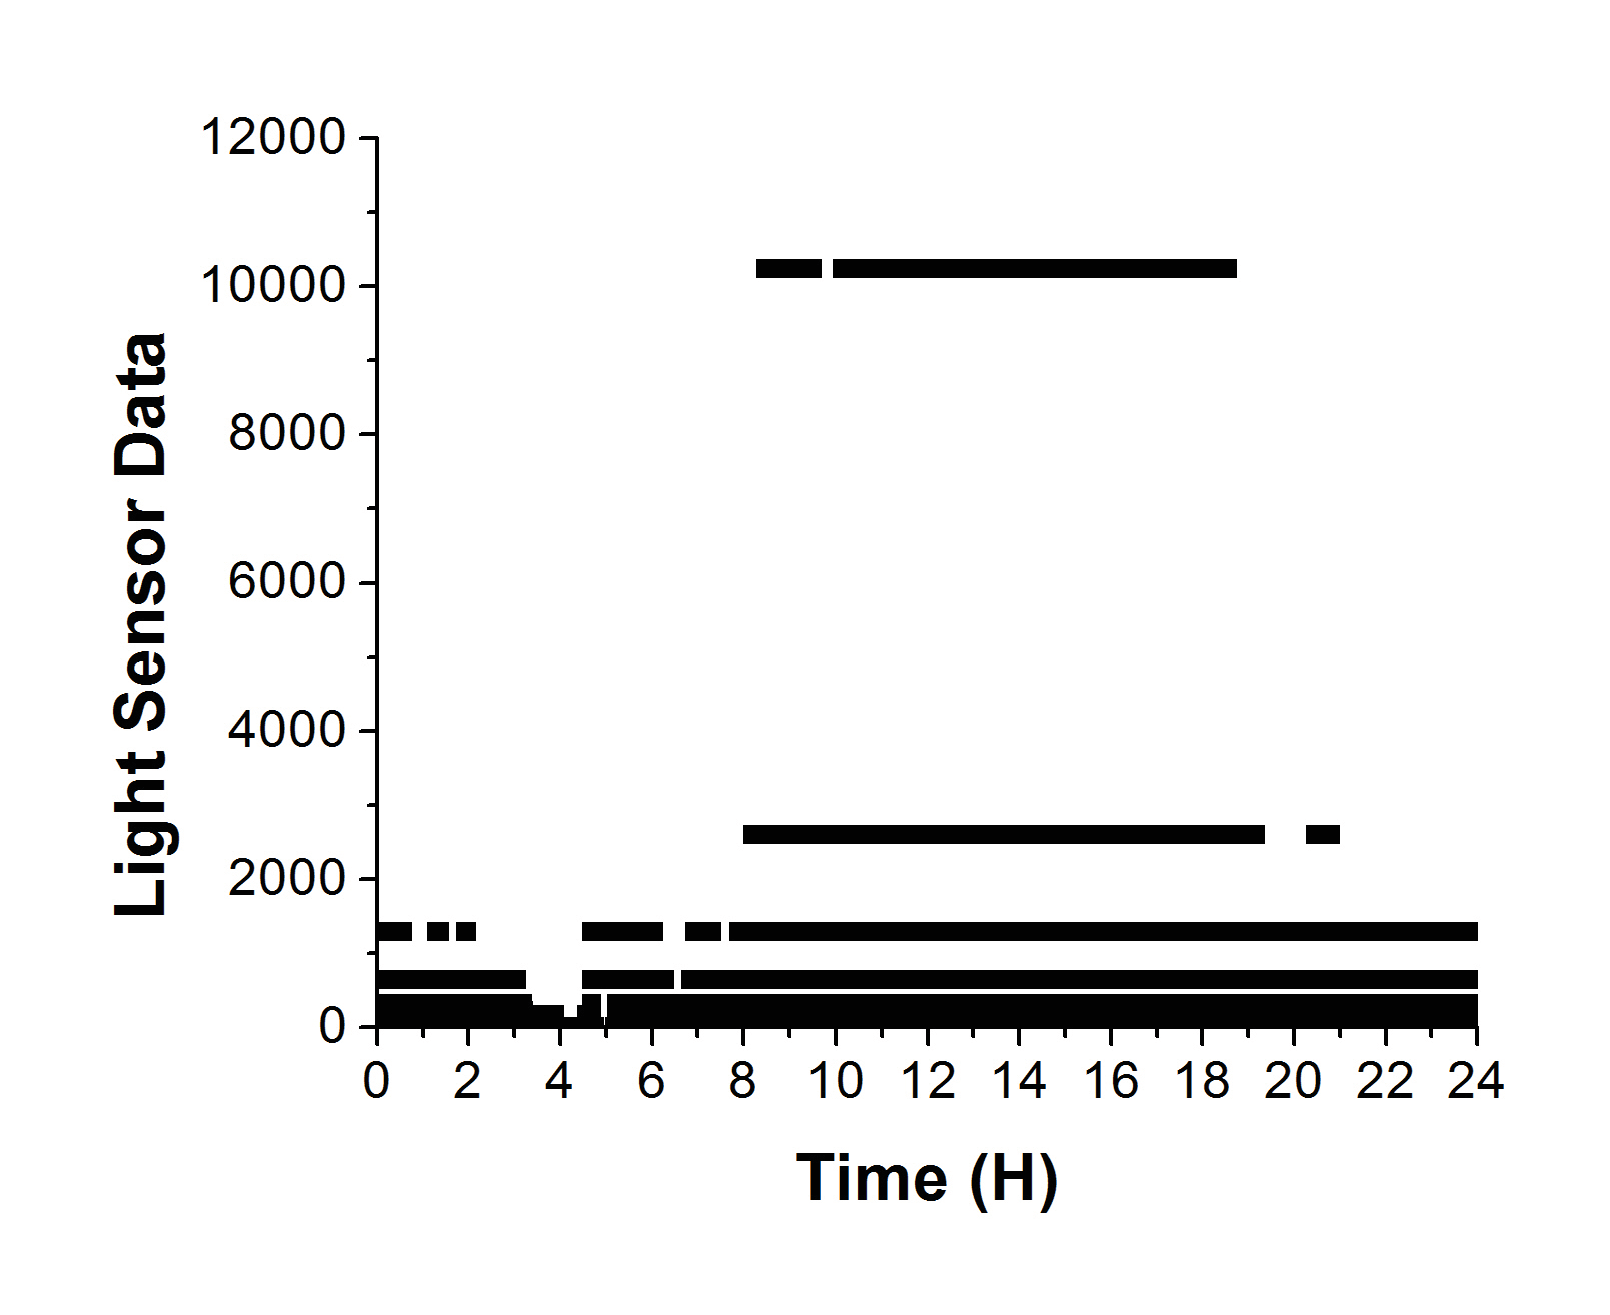
\includegraphics[width=3.5in]{graphs/Figure14.eps}}
\caption{Light Sensor Data Distribution on Tuesday} 
\label{fig:light_tuesday}
\end{figure}

\begin{table}[ht] 
\caption{PROXIMITY VARIATION ON TUESDAY DAYTIME} 
\centering  
\begin{tabular}{cccc}
\hline
 & Proximity Detected & Maybe Detected & None\\[0.5ex] 
\hline\hline 8am-11am & 90 & 89 & 14\\
\hline 11am-2pm & 101 & 82 & 10\\
\hline 2pm-5pm & 89 & 97 & 7\\
\hline 5pm-8pm & 84 & 98 & 11\\
\hline
\end{tabular}
\label{table:tuesday} 
\end{table}


Figure~\ref{fig:bt_tuesday} reflects the distribution of Bluetooth RSSI values on that day. The most frequently value is around -75dBm which is similar as concluded in Figure~\ref{fig:multiphones}. As revealed in Section~\ref{sec:exp}, when RSSI value is smaller than -75dBm, it has a relatively low probability that the two phones are in face-to-face proximity. 
Critically, a method such as the one in ~\cite{Nathan3,Nathan1} would misdetect such interactions. Based on both Bluetooth RSSI values and light sensor values, our model can improve the accuracy of face-to-face proximity indication. 

\begin{figure}[h!tbp]
\centering
{\includegraphics[width=3.5in]{graphs/Figure15.eps}}
\caption{Bluetooth RSSI Values Distribution on Tuesday} 
\label{fig:bt_tuesday}
\end{figure}

\subsection{Proximity in small group}

\emph{Football Game Day: }
In 2011, the university had a football game with Air Force which lasted for four hours. There were 126 students among the 196 that watched the game in the stadium and we gathered 56710 Bluetooth records in the database. In Figure~\ref{fig:018},  we select one participant \textit{S018} and show the detected phones around that student through Bluetooth during the 4 hour period. For every five minutes, if any other phone is detected we add its corresponding ID in that time slot. There are total 48 time slots and with several students always together with the student in the game. Similarly, we explore one of those nearby students \textit{S077} to validate symmetric detection in Figure~\ref{fig:077}. These two figures further show that it is practical to use Bluetooth to detect people around. 
\begin{figure}[h!tbp]
\centering
{\includegraphics[width=3.5in]{graphs/Figure16.eps}}
\caption{\textit{S018} Data on Game Day} 
\label{fig:018}
\end{figure} 

\begin{figure}[h!tbp]
\centering
{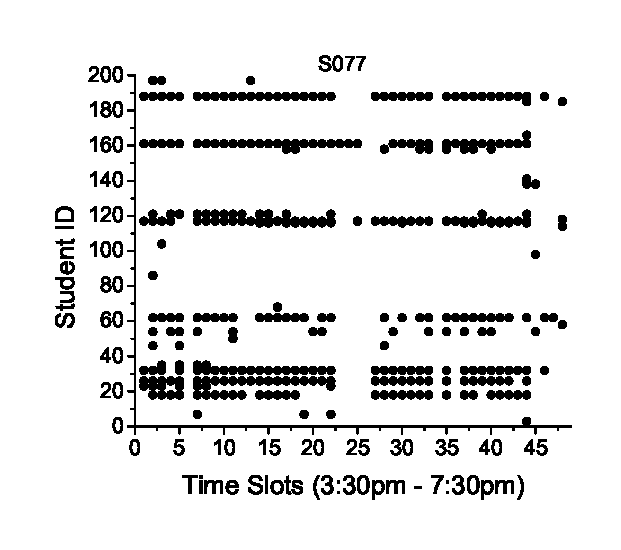
\includegraphics[width=3.5in]{graphs/Figure17.eps}}
\caption{\textit{S077} Data on Game Day} 
\label{fig:077}
\end{figure} 

Figure~\ref{fig:018} shows the detected students around without any restriction of Bluetooth RSSI values. In order to get list of the students in face-to-face proximity, we need to utilize the proximity estimation model to refine the results. Combined with light sensor data and method of data smoothing, the probability of proximity is calculated for the filtration. With RA of 45\%, Figure~\ref{fig:018_80} shows the filtered results which is more accurate to indicate the people who is in the face-to-face conversation range with the participant in the game. Compared with Figure~\ref{fig:018}, it is much more clear to find other devices kept close with the participant during the game. 

We analyzed the symmetry between \textit{S018} and \textit{S077} in a more accurate way with proximity estimation model. In section~\ref{sec:exp} we discussed the symmetry of Bluetooth RSSI values between two phones and the values are almost the same when the noisy and interference is relatively low. Does such symmetry still exist when more than two phones are nearby? We look into the data reported on the game day again to check whether the symmetry between \textit{S018} and \textit{S077} still exists or not. Figure~\ref{fig:symmetry} includes the data from both \textit{S018} and \textit{S077} with RA equals to 45\% and (018,077) means that \textit{S018} detected \textit{S077} was in the face-to-face range in the specific time slot. Due to the interference from other phones with Bluetooth, the values are not exactly symmetric in the four hours. There is nearly 40\% of the time when such proximity detection is not symmetric. 

\begin{figure}[h!tbp]
\centering
{\includegraphics[width=3.5in]{graphs/Figure18.eps}}
\caption{\textit{S018} Data on Game Day with Proximity Estimation Model} 
\label{fig:018_80}
\end{figure}

\begin{figure}[h!tbp]
\centering
{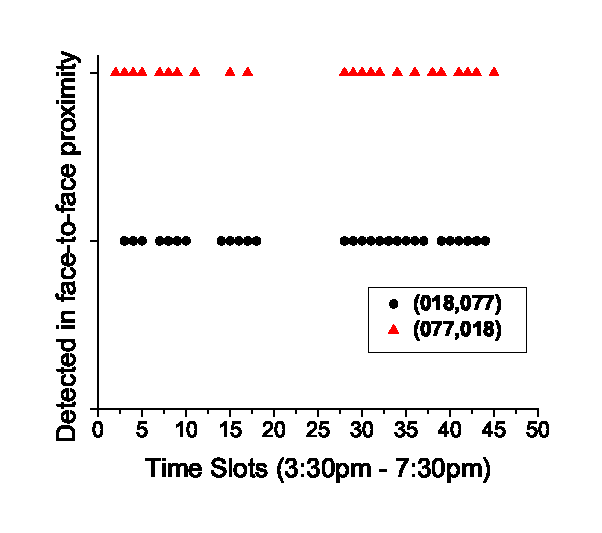
\includegraphics[width=3.5in]{graphs/Figure19.eps}}
\caption{Symmetry Analysis of Data on Game Day} 
\label{fig:symmetry}
\end{figure}

\emph{Weekday: }
In this part, we analyzed the data recorded during weekdays, such as class time and lunch hours, and compared it with the data on game days. During the football game, most of the freshmen sit in the same student section and it is highly possible to detect more than 10 people around him/her at one time slot. However, when students are in class or having lunch, the data becomes reasonably sparse. Compared to more than fifty thousand records in the game, we recorded 6408 records on Oct 11th 2011 (Tuesday) from 9am to 1pm. Figure~\ref{fig:018_class} illustrates the data reported by the same phone \textit{S018} during this period. Obviously, the chance to meet other students (related to this project) in class or during the lunch time is relatively low. In \textit{S018}'s case, he/she only met with two other students within a direct-communication distance in class and four during the lunch time. 

\begin{figure}[h!tbp]
\centering
{\includegraphics[width=3.5in]{graphs/Figure20.eps}}
\caption{\textit{S018} Data on Weekday with Proximity Estimation Model} 
\label{fig:018_class}
\end{figure}

\begin{figure}[h!tbp]
\centering
{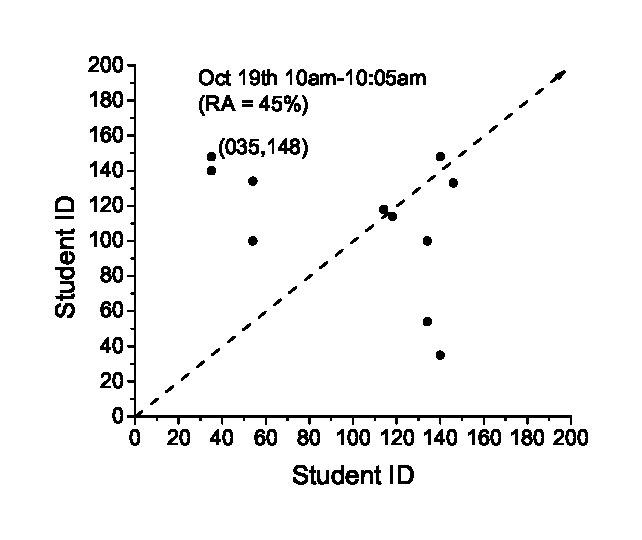
\includegraphics[width=3.5in]{graphs/Figure21.eps}}
\caption{Fallbreak Data with Proximity Estimation Model} 
\label{fig:fallbreak}
\end{figure}

\emph{Fall Break: }
During the fall break (from Oct 17th to Oct 23rd), most students went home and we got relatively less data. Take the data of Oct 19th for example, we got 4373 records in the whole day and only 26 devices detected other devices in the project in face-to-face proximity. We used the proximity estimation model and the same RA to analyze the results we got on Oct 19th between 10am and 10:05am. Figure~\ref{fig:fallbreak} shows the proximity status among students in this specific time slot. There are in total 11 samples collected during the 5-minutes period and (035, 148) means device \textit{S035} detected \textit{S148} was in the face-to-face proximity. Since there is less interference, the symmetry is maintained as observed in Section~\ref{sec:exp}. In Figure~\ref{fig:fallbreak}, more than 70\% values are symmetric. Compared with self-reporting method, our proximity estimation model is a more reliable and effective method to detect face-to-face proximity in daily life. 

\section{Summary}
In this section, our presented work validates the usage of Bluetooth as a tool for face-to-face proximity detection and makes the following contributions:
\begin{itemize}
\item We demonstrate the viability of using Bluetooth for the purposes of face-to-face proximity estimation and propose a proximity estimation model with appropriate smoothing and consideration of a wide variety of typical environments. 
\item We study the relationship between the value of Bluetooth RSSI and distance based on empirical measurements and compare the results with the theoretical results using the radio propagation model. 
\item Based on the monitoring system, we are able to use the proximity estimation model across several real-world cases to provide high accurate determination of face-to-face interaction distance.
\end{itemize}
Based the empirical Bluetooth RSSI results, we further study the potential of opportunistic relaying when two devices are in close proximity in Chapter~\ref{chap:opp_relay}. 